\subsection{Fourier series and trigonometric polynomials}
Instead of arbitrary $\phi_i$ substitute $e^{i \pi k}$ to \eqref{eq:linear_expansion}:
\begin{equation*}
	\begin{multlined}
		S_K(x) = \beta_0 + \sum_{i = 1}^K \beta_i e^{i \pi k x} \implies S(x) = a_0 + \sum_{i = 1}^K \left (a_i cos(\pi k x) + b_i sin(\pi k x) \right ) \\
	\end{multlined}
\end{equation*}
This set of functions is orthogonal on the considered interval:
\begin{equation*} 
	\int_{-\pi}^{\pi} e^{i \pi k x} e^{i \pi l x} = 2\pi \delta_k^l 
\end{equation*}
Estimating $ a_n $ and $ b_n $ for some function $ f $ is a simple process. First you need to determine the discrepancy - $ R (x) = f (x) - S_K (x) $ between the function and its expansion, after that the resulting discrepancy must be integrated by its square over the region and use the least squares method:
\begin{equation*}
	\begin{multlined}
		\mathcal{L} = \int_{\Omega} R(x)^2 d\Omega = \int_{\Omega} \left ( f(x) - S_K(x) \right )^2 d\Omega = \\ = \int_{\Omega} f(x)^2 d\Omega - 2 \int_{\Omega} S_K(x) f(x) d\Omega + \int_{\Omega} S_K(x)^2 d\Omega = \\ = \int_{\Omega} f(x)^2 d\Omega - 2 \int_{\Omega} \left [ a_0 + \sum_{i = 1}^K \left (a_i cos(\pi k x) + b_i sin(\pi k x) \right ) \right ] f(x) d\Omega + \\ +  \int_{\Omega} \left [ a_0 + \sum_{i = 1}^K \left (a_i cos(\pi k x) + b_i sin(\pi k x) \right ) \right ]^2 d\Omega
	\end{multlined}
\end{equation*}
The least squares method itself involves using the derivatives of the resulting integral residual for each parameter that you want to evaluate, respectively:
\begin{equation}
 	\begin{multlined}
 		\begin{cases}
 			\dfrac{\partial }{\partial a_n} \mathcal{L} = \dfrac{\partial \mathcal{L}}{\partial S_K(x)} \dfrac{\partial S_K(x)}{\partial a_n}  = -2 {\displaystyle \int_{\Omega}} f(x) cos(\pi k x) d\Omega + -2 {\displaystyle \int_{\Omega}} S_K(x) cos(\pi k x) d\Omega \\[20pt]
 			\dfrac{\partial }{\partial b_n} \mathcal{L} = \dfrac{\partial \mathcal{L}}{\partial S_K(x)} \dfrac{\partial S_K(x)}{\partial b_n} = -2 {\displaystyle \int_{\Omega}} f(x) sin(\pi k x) d\Omega + -2 {\displaystyle \int_{\Omega}} S_K(x) sin(\pi k x) d\Omega \\[20pt]
 			\dfrac{\partial }{\partial a_0} \mathcal{L} = \dfrac{\partial \mathcal{L}}{\partial S_K(x)} \dfrac{\partial S_K(x)}{\partial a_0}  = -2 {\displaystyle \int_{\Omega}} f(x) d\Omega + 2 |\Omega| a_0 \\[20pt]
 		\end{cases}
 	\end{multlined}
 	% \mathcal{L} = \int_{\Omega} R(x)^2 d\Omega
\end{equation}
The main part of the calculations is absent and provided here \cite{fourierintro}. In addition, there is a convergence analysis of the coefficients, in sense of pointwise, and $L_2$ norm. The final result for the coefficients is:
\begin{equation}
	\begin{cases}
		a_0 = \dfrac{{\displaystyle \int_{\Omega}} f(x) d\Omega }{2 | \Omega |} \\[20pt]
		a_n = \dfrac{{\displaystyle \int_{\Omega}} f(x) cos(\pi k x) d\Omega}{| \Omega |} \\[20pt]
		b_n = \dfrac{{\displaystyle \int_{\Omega}} f(x) sin(\pi k x) d\Omega}{| \Omega |} \\[20pt]
	\end{cases}
\end{equation}

For example, consider the function $y = sin(x) + x$ and at the figure \ref{fig:fourier_demo} the results. It can be seen that with a relatively small amount of the terms the approximation good. With 3 terms the approximation error\footnote{Here, the approximation error is the loss function and concrete - mean squared error between the known values and Fourier expansion. There is a pointwise loss value, where the error calculation includes the finite number of nodes and integral loss value, where the residual integrates over the all domain.} is 0.565, 5 terms - 0.005 and 10 terms is 0.002.
\begin{figure}[h]
	\centering
	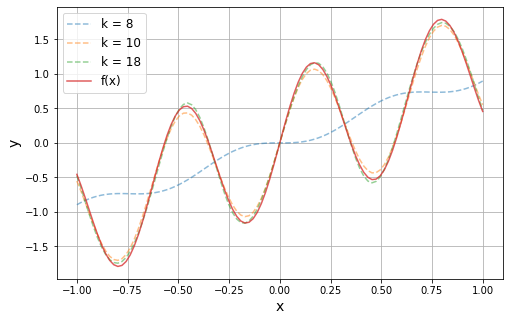
\includegraphics[width=\textwidth]{images/chapter2/fourier_demo.png}
	\caption{Example of function expansion into the Fourier series with 3, 10, 18 terms}
	\label{fig:fourier_demo}
\end{figure}

\subsubsection{The strong sides of Fourier expansion}
Two important theorems help to use the Fourier decomposition to construct a future approximation. Each of them can be found with evidence in \cite{fourierintro}.
\newtheorem{theorem}{Theorem}[chapter]
\begin{theorem}
\label{convergence-l2-norm}
If $f$ belongs to $L^{2}(\left[-\pi ,\pi \right])$ then $S_k$ converges to $f$ in $L^{2}(\left[-\pi ,\pi \right])$, that is, $\|S_K - f\|_{2}$ converges to 0 as $N \rightarrow \infty$.
\end{theorem}
\begin{theorem}
\label{convergence-pointwise}
If $f$ belongs to $C^1(\left[-\pi ,\pi \right])$ then $S_k$ converges to $f$ uniformly (and hence also pointwise).
\end{theorem}
The proofs of theorems well provided here \cite{fourierintro}. And an additional fact, Fourier coefficients of any integrable function tend to zero.

In the case where the non-least squares method will be used, the problem may have another solution - a set of coefficients, which in the general case will not be Fourier series expansion. The reason is that for a predetermined number of terms in a series, naturally, based on them, get the best approximation without looking at the fact that in theory their number is infinite. If the gradient-based method is to be used, it is important to use the results obtained for the regression, which guarantee the uniqueness of the maximum with accuracy, then the rearrangement of the parameters in places - regularization. Let there be a vector $ x $, a vector of weights $ w $, and an offset $ b $:
\begin{equation*}
	y = w^T x + b, \quad z = cos(y) = cos \left [ w^T x + b \right ]
\end{equation*}
In the general case, we use the condition of orthogonality of the functions $y_i$:
\begin{equation*}
	\begin{split}
		\int_{\Omega} y_i \cdot y_j d\Omega = \int_{\Omega} cos \left [ w_i x_i + b_i \right ] \cdot cos \left [ w_j x_j + b_j \right ] d\Omega = \\[10pt] = \dfrac{sin(w_i - w_j) + b_i - b_j}{2 w_i - 2 w_j} + \dfrac{sin(w_i + w_j) + b_i + b_j}{2 w_i + 2 w_j} \rightarrow \delta_k^l
	\end{split}
\end{equation*}

And it turns out that adding the term $\mathcal{L}_{\text{regularization}}$ to the loss function, during the optimization process, the task will converge in addition to the solution, as well as to the true coefficients in the expansion.

\begin{equation}
	\label{eq:regularization_criterion_fourier}
	\mathcal{L}_{\text{regularization}} = \left [ \dfrac{sin(w_i - w_j) + b_i - b_j}{2 w_i - 2 w_j} + \dfrac{sin(w_i + w_j) + b_i + b_j}{2 w_i + 2 w_j} - \delta_k^l \right ]^2
\end{equation}

or in matrix form:
\begin{equation}
	\label{eq:regularization_criterion_fourier_matrix}
	\mathcal{L}_{\text{regularization}} = \left [ \dfrac{sin(W - W^T) + B - B^T}{2 W - 2 W^T} + \dfrac{sin(W + W^T) + B + B^T}{2 W + 2 W^T} - I \right ]_F
\end{equation}
, where $ \| A \|_F $ - Frobenius norm of $A$:
\begin{equation*}
	 \| A \|_F = \sqrt{ \sum_{i, j} A_{ij}^2 }
\end{equation*}

\begin{figure}
	\centering
	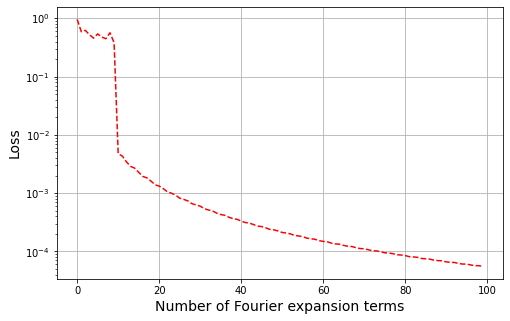
\includegraphics[width=\textwidth]{images/chapter2/fourier_quality.png}
	\caption{Illustration of the theorems \ref{convergence-l2-norm}, \ref{convergence-pointwise} for the function from the previous example}
	\label{fig:fourier_quality}
\end{figure}